\documentclass[tikz,border=8pt]{standalone}
\usepackage{amsmath,amssymb}
\usetikzlibrary{arrows.meta,calc,decorations.pathreplacing,patterns,shapes.geometric,positioning,shadings,plotmarks}

\definecolor{coreblue}{HTML}{D9ECFF}
\definecolor{cladgray}{HTML}{EEEEEE}
\definecolor{ergreen}{HTML}{C8E6C9}
\definecolor{rayred}{HTML}{C0392B}
\definecolor{pumpviolet}{HTML}{6A1B9A}

\begin{document}
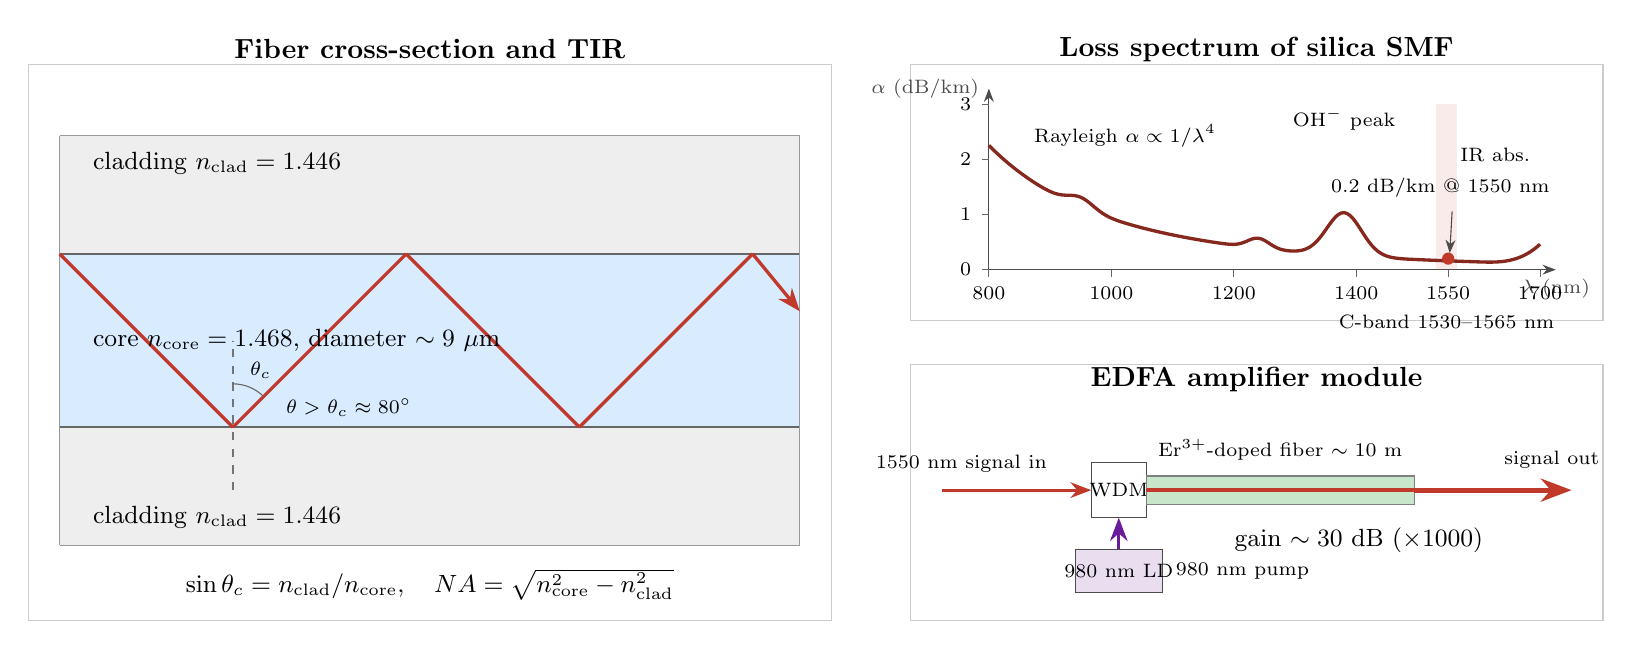
\begin{tikzpicture}[>=Stealth,font=\small]

% =====================================================
% Layout:
%  LEFT : TIR ray tracing  (x in [0,10],  y in [0,7])
%  TOP RIGHT    : loss vs wavelength (shift to (11.2,3.8))
%  BOTTOM RIGHT : EDFA schematic     (shift to (11.2,0))
% =====================================================

% ======================================================
% PANEL 1 : Fiber cross-section with TIR zigzag
% ======================================================
\begin{scope}[shift={(0,0)}]
  \node[font=\bfseries] at (5,7.2) {Fiber cross-section and TIR};

  % Fiber geometry (numeric constants to avoid macro coordinate issues)
  % Core: y in [2.4, 4.6], cladding top: [4.6, 6.1], cladding bottom: [0.9, 2.4]
  \fill[cladgray] (0.3,4.6) rectangle (9.7,6.1);
  \fill[cladgray] (0.3,0.9) rectangle (9.7,2.4);
  \fill[coreblue] (0.3,2.4) rectangle (9.7,4.6);

  % Interfaces (core-cladding boundaries) - heavier
  \draw[black!60,thick] (0.3,4.6) -- (9.7,4.6);
  \draw[black!60,thick] (0.3,2.4) -- (9.7,2.4);

  % Outer boundaries
  \draw[black!40] (0.3,6.1) -- (9.7,6.1);
  \draw[black!40] (0.3,0.9) -- (9.7,0.9);
  \draw[black!40] (0.3,0.9) -- (0.3,6.1);
  \draw[black!40] (9.7,0.9) -- (9.7,6.1);

  % Zigzag ray: start top-left, bounce four times, exit right
  % Endpoints on interfaces (y = 2.4 or 4.6), equal-length segments
  \draw[rayred,very thick] (0.3,4.6) -- (2.5,2.4);
  \draw[rayred,very thick] (2.5,2.4) -- (4.7,4.6);
  \draw[rayred,very thick] (4.7,4.6) -- (6.9,2.4);
  \draw[rayred,very thick] (6.9,2.4) -- (9.1,4.6);
  \draw[rayred,very thick,->] (9.1,4.6) -- (9.7,3.87);

  % Normal dashed line at first TIR bounce (x=2.5, y=2.4)
  \draw[dashed,black!55] (2.5,1.6) -- (2.5,3.5);

  % Angle arc theta_c between normal (upward) and ray going up-right
  \draw[black!60] (2.5,2.4) ++(90:0.55) arc (90:45:0.55);
  \node[font=\scriptsize] at (2.85,3.12) {$\theta_c$};

  % Greater-than-critical note
  \node[font=\scriptsize,anchor=west] at (3.05,2.65)
    {$\theta > \theta_c \approx 80^{\circ}$};

  % Labels for core and cladding
  \node[anchor=west,font=\small] at (0.6,5.75)
    {cladding  $n_{\mathrm{clad}} = 1.446$};
  \node[anchor=west,font=\small] at (0.6,1.25)
    {cladding  $n_{\mathrm{clad}} = 1.446$};
  \node[anchor=west,font=\small] at (0.6,3.5)
    {core  $n_{\mathrm{core}} = 1.468$, diameter $\sim 9\ \mu$m};

  % Formula band underneath panel
  \node[font=\small] at (5,0.4)
    {$\sin\theta_c = n_{\mathrm{clad}}/n_{\mathrm{core}},\quad
      NA = \sqrt{n_{\mathrm{core}}^{2}-n_{\mathrm{clad}}^{2}}$};

  % Panel frame
  \draw[gray!40] (-0.1,-0.05) rectangle (10.1,7);
\end{scope}

% ======================================================
% PANEL 2 : Loss vs wavelength (top right)
% ======================================================
\begin{scope}[shift={(11.2,3.8)}]
  % Frame
  \draw[gray!40] (-0.1,-0.05) rectangle (8.7,3.2);

  % Title
  \node[font=\bfseries] at (4.3,3.4) {Loss spectrum of silica SMF};

  % Plot area
  \def\pxL{0.9}
  \def\pxR{7.9}
  \def\pyB{0.6}
  \def\pyT{2.7}

  % Axes
  \draw[->,black!70] (\pxL,\pyB) -- (8.1,\pyB)
      node[anchor=north,font=\scriptsize] {$\lambda$ (nm)};
  \draw[->,black!70] (\pxL,\pyB) -- (\pxL,2.9)
      node[anchor=east,font=\scriptsize] {$\alpha$ (dB/km)};

  % X ticks
  \foreach \lam/\lab in {800/800,1000/1000,1200/1200,1400/1400,1550/1550,1700/1700}{%
    \pgfmathsetmacro{\xx}{\pxL + (\lam-800)/900 * (\pxR-\pxL)}
    \draw[black!60] (\xx,\pyB) -- (\xx,\pyB-0.09);
    \node[font=\scriptsize,anchor=north] at (\xx,\pyB-0.09) {\lab};
  }
  % Y ticks (0..3 dB/km)
  \foreach \val in {0,1,2,3}{%
    \pgfmathsetmacro{\yy}{\pyB + \val/3 * (\pyT-\pyB)}
    \draw[black!60] (\pxL,\yy) -- (\pxL-0.09,\yy);
    \node[font=\scriptsize,anchor=east] at (\pxL-0.1,\yy) {\val};
  }

  % C-band shading first (so curve draws over it)
  \pgfmathsetmacro{\xcL}{\pxL + (1530-800)/900 * (\pxR-\pxL)}
  \pgfmathsetmacro{\xcR}{\pxL + (1565-800)/900 * (\pxR-\pxL)}
  \fill[rayred,opacity=0.10] (\xcL,\pyB) rectangle (\xcR,\pyT);

  % Curve: Rayleigh baseline + OH peaks + IR rise
  % alpha(lam) = 0.16*(1550/lam)^4
  %            + OH peaks (gaussians at 1380, 1240, 950)
  %            + IR rise for lam>1600 (cubic)
  \draw[rayred!70!black,line width=1.2pt,smooth,samples=181,domain=800:1700,variable=\l]
    plot ({\pxL + (\l-800)/900 * (\pxR-\pxL)},
          {\pyB + ( 0.16*pow(1550/\l,4)
                  + 0.78*exp(-pow((\l-1380)/40,2))
                  + 0.18*exp(-pow((\l-1240)/25,2))
                  + 0.18*exp(-pow((\l-950)/30,2))
                  + (\l>1600 ? 0.18*pow((\l-1600)/80,3) : 0)
                  )/3 * (\pyT-\pyB) });

  % Highlight 1550 nm minimum
  \pgfmathsetmacro{\xFive}{\pxL + (1550-800)/900 * (\pxR-\pxL)}
  \pgfmathsetmacro{\yFive}{\pyB + 0.2/3 * (\pyT-\pyB)}
  \fill[rayred] (\xFive,\yFive) circle (2.2pt);
  \draw[->,black!70] (\xFive+0.05,\yFive+0.6) -- (\xFive+0.02,\yFive+0.07);
  \node[font=\scriptsize,anchor=south] at (\xFive-0.1,\yFive+0.65)
    {$0.2$ dB/km @ $1550$ nm};

  % Region labels
  \node[font=\scriptsize,anchor=west] at (1.35,2.30)
    {Rayleigh $\alpha \propto 1/\lambda^{4}$};
  \pgfmathsetmacro{\xOH}{\pxL + (1380-800)/900 * (\pxR-\pxL)}
  \node[font=\scriptsize,anchor=south] at (\xOH,2.25) {OH$^{-}$ peak};
  \node[font=\scriptsize,anchor=south east] at (7.9,1.85) {IR abs.};
  \node[font=\scriptsize,anchor=north] at ({(\xcL+\xcR)/2},\pyB-0.45) {C-band 1530--1565 nm};
\end{scope}

% ======================================================
% PANEL 3 : EDFA schematic (bottom right)
% ======================================================
\begin{scope}[shift={(11.2,0)}]
  % Frame
  \draw[gray!40] (-0.1,-0.05) rectangle (8.7,3.2);
  \node[font=\bfseries] at (4.3,3.0) {EDFA amplifier module};

  % Signal fiber layout
  \def\yf{1.6}
  \def\xfA{0.3}
  \def\xfB{2.2}
  \def\xfC{2.9}
  \def\xfD{6.3}
  \def\xfE{8.3}

  % Input signal fiber (thin)
  \draw[rayred,line width=1.0pt,->] (\xfA,\yf) -- (\xfB,\yf);

  % WDM coupler
  \draw[black!70,fill=white] (\xfB,\yf-0.35) rectangle (\xfC,\yf+0.35);
  \node[font=\scriptsize] at (2.55,\yf) {WDM};

  % Er-doped section (green)
  \fill[ergreen] (\xfC,\yf-0.18) rectangle (\xfD,\yf+0.18);
  \draw[black!50] (\xfC,\yf-0.18) rectangle (\xfD,\yf+0.18);
  \draw[rayred,line width=1.4pt] (\xfC,\yf) -- (\xfD,\yf);

  % Output signal (thick) with arrow
  \draw[rayred,line width=1.8pt,->] (\xfD,\yf) -- (\xfE,\yf);

  % Pump laser diode box
  \draw[black!70,fill=pumpviolet!15] (2.0,0.3) rectangle (3.1,0.85);
  \node[font=\scriptsize] at (2.55,0.575) {980 nm LD};
  % Pump arrow into WDM
  \draw[pumpviolet,line width=1.2pt,->] (2.55,0.85) -- (2.55,\yf-0.35);

  % Labels
  \node[font=\scriptsize,anchor=south] at (\xfA+0.25,\yf+0.1) {1550 nm signal in};
  \node[font=\scriptsize,anchor=south] at (\xfE-0.25,\yf+0.15) {signal out};
  \node[font=\scriptsize,anchor=south] at ({(\xfC+\xfD)/2},\yf+0.25)
    {Er$^{3+}$-doped fiber $\sim 10$ m};
  \node[font=\scriptsize,anchor=west] at (3.15,0.575) {980 nm pump};

  % Gain annotation
  \node[font=\small,anchor=north] at ({(\xfC+\xfE)/2},\yf-0.35)
    {gain $\sim 30$ dB ($\times 1000$)};
\end{scope}

\end{tikzpicture}
\end{document}
